\section{Layout}

The layout algorithm, determining the positions of sets and events within them,  consists of four steps. First, the vertical ordering of sets is computed to ensure that two sets that share events are next to each other wherever possible. Then, sets are further divided into layers, and events are assigned to these layers according to their memberships. After that, the position and length of each event are computed, within the given display space. Finally, layers are compacted to remove any gaps between them, before their sizes are adjusted to yield a consistent level of detail across all sets. 

\subsection{Sets Ordering}
\label{sec:set-ordering}
The set ordering algorithm aims to maximize the number of events shared by neighboring sets. This can be mapped to a graph path problem. Given a list of sets $S=\{s_1, s_2, \dotsc, s_n\}$, an undirected graph $G = (V,E)$ is created with each vertex $v_i$ representing a set $s_i \in S$. Two vertices $v_i$ and $v_j$ are connected if $s_i$ and $s_j$ share an event. The weight of edge $e_{ij}$ is the number of events shared by $s_i$ and $s_j$. Finding a set order with the maximum number of events shared by neighboring sets is equivalent to finding a path with the maximum weight connecting all vertices in $G$. This longest path problem is known to be NP-hard. The number of sets we plan to support is constrained by the number of colors that human can easily distinguish when they are shown together; and they are only around 12 colors~\cite{Munzner2014}. Therefore, we decide to use a brute-force approach to find the optimal solution.

\subsection{Layer Layout}
% Requirements
This algorithm positions all the events within a layer. Its inputs include:
\begin{itemize}
	\item The events belonging to the layer with their \emph{label} and \emph{time} values.
	\item The maximum width and height of the layer.
\end{itemize}
The outputs are event locations within the constrained display area, optimizing for the following criteria:
\begin{description}
	\item[Completeness] measuring how much event labels are visible. More specifically, we define the \emph{completeness ratio} as:
	$\theta = \frac{\alpha \cdot |E_c| + \beta \cdot |E_t|}{|E|}$, where $|E_c|$ is the number of complete events, $|E_t|$ is the number of trimmed events, and $|E|$ is the number of all events. $\alpha$ and $\beta$ are the coefficients to indicate how strongly complete events and trimmed events contribute to the overall content richness of the layer, respectively. We practically set $\alpha=1$ and $\beta=0.5$.
	
	\item[Traceability] measuring how easy it is to follow the events within a layer chronologically. Events happened close in time should have small changes in their row levels to facilitate the reading flow. More specifically, we define the \emph{traceability ratio} as:
	$\gamma=\frac{\sum\limits_{i=1}^{|E|}(|l_{i+1} - l_i|)}{|E|-1}$	, where $|E|$ is the number of all events within the layer and $l_i$ is the row level of event $e_i$. 	
\end{description}

The horizontal position of an event is fixed by its time. The layout algorithm decides on which row to position an event; i.e., vertical position,  and the level of detail for its label.

\subsubsection{Completeness Algorithm}
Starting with an empty layer, the algorithm processes events chronologically. An event is located at the possibly lowest row where it does not overlap with any other events. If such a row does not exist, one of the earlier located events is trimmed to make space for it. Among these events, the one with the least text being trimmed is selected. However, if the label space of that event is too short for a single word after trim, it will combine with the current event to form a new aggregated event labeled ``2 events''. Aggregated events cannot be trimmed, thus if a new event overlaps with them, it will be added into the existing aggregate. For example, a new event that overlaps with a ``2 events'' aggregated event will be grouped together producing the ``3 events'' aggregate. 

The completeness algorithm maximizes the number of complete events $|E_c|$ and trimmed events $|E_t|$, thus yielding a maximum completeness ratio $\theta$. However, this algorithm does not optimize traceability because an event is located in the possibly lowest row disregarding the row level of its preceding event.

\subsubsection{Traceability Algorithm}
To improve traceability, the algorithm inserts a new event at the same row as its preceding event. If they overlap, the preceding event is trimmed to make space for the currently adding one. We define the \emph{trim ratio} of an event as the ratio of the remaining text length to its original length. An event can only be trimmed if the resulting trim ratio is greater than a minimum threshold $t_{min}$, where $0\leq t_{min} \leq 1$. This value determines how much completeness can be traded for traceability. If the resulting trim ratio is smaller than $t_{min}$, the event moves up or down, up to $r_{max}$ rows on both sides, to find a satisfied row. $r_{max}$ decides how far, in terms of row level difference, an event can be from the preceding event, which essentially trades traceability for completeness. If no suitable row can be found within $\pm r_{max}$ rows, the currently adding event returns to the level of its preceding event, which is then trimmed or aggregated with the preceding event as in the completeness algorithm.

Figure~\ref{fig:traceability} shows an example of these two algorithms. Both layer layout algorithms run in linear time in terms of the number of events, because during the event insertion, the completeness algorithm checks up to a constant number -- the layer height -- of times, and the traceability algorithm checks at most ($2 \times r_{max}+1$) rows.

\begin{figure}[!htb]
\centering
	\subcaptionbox{Completeness algorithm: $\theta=1$, \\$\gamma=5/3$.}{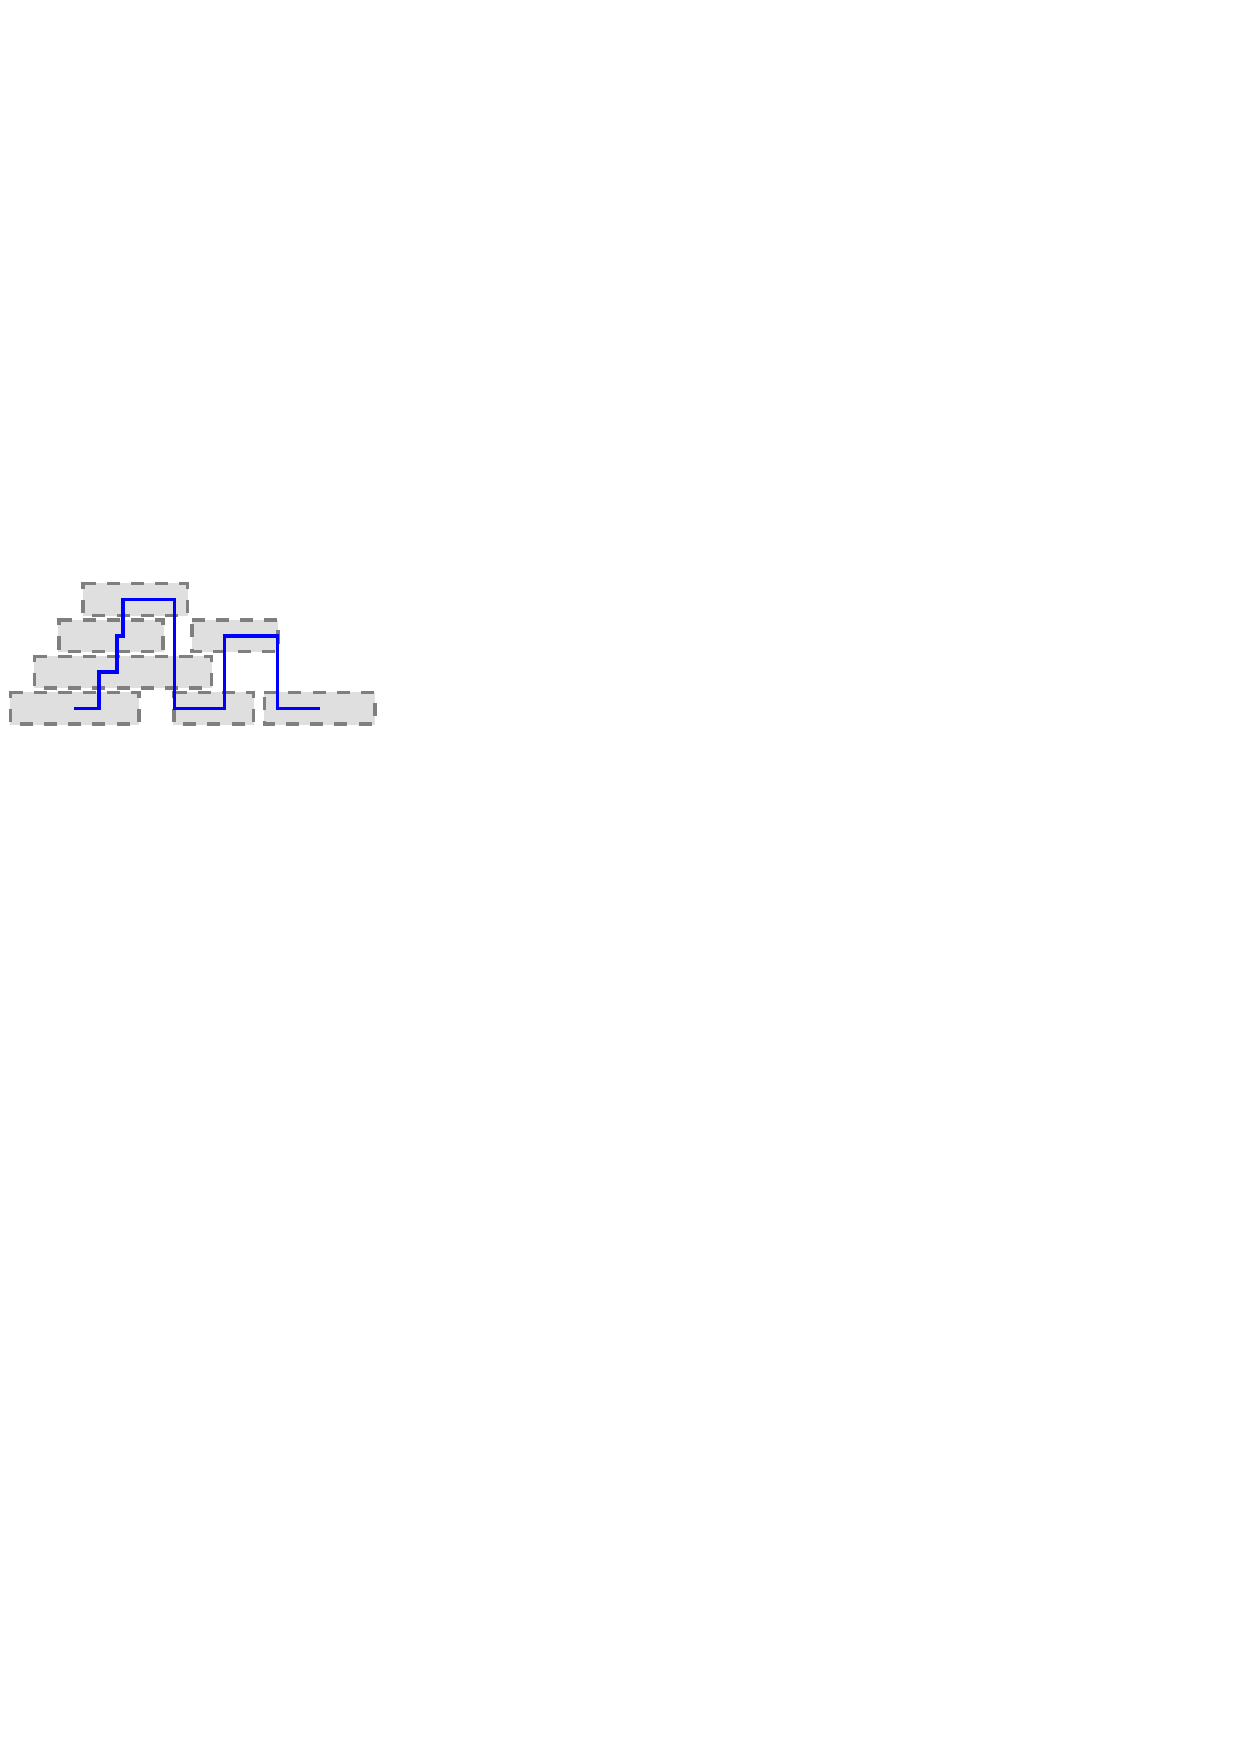
\includegraphics[width=.47\linewidth]{figure9a}}
	\hfill
	\subcaptionbox{Traceability algorithm ($t_{min}=0.5$, $r_{max}=1$): $\theta=6/7$, $\gamma=2/3$.}{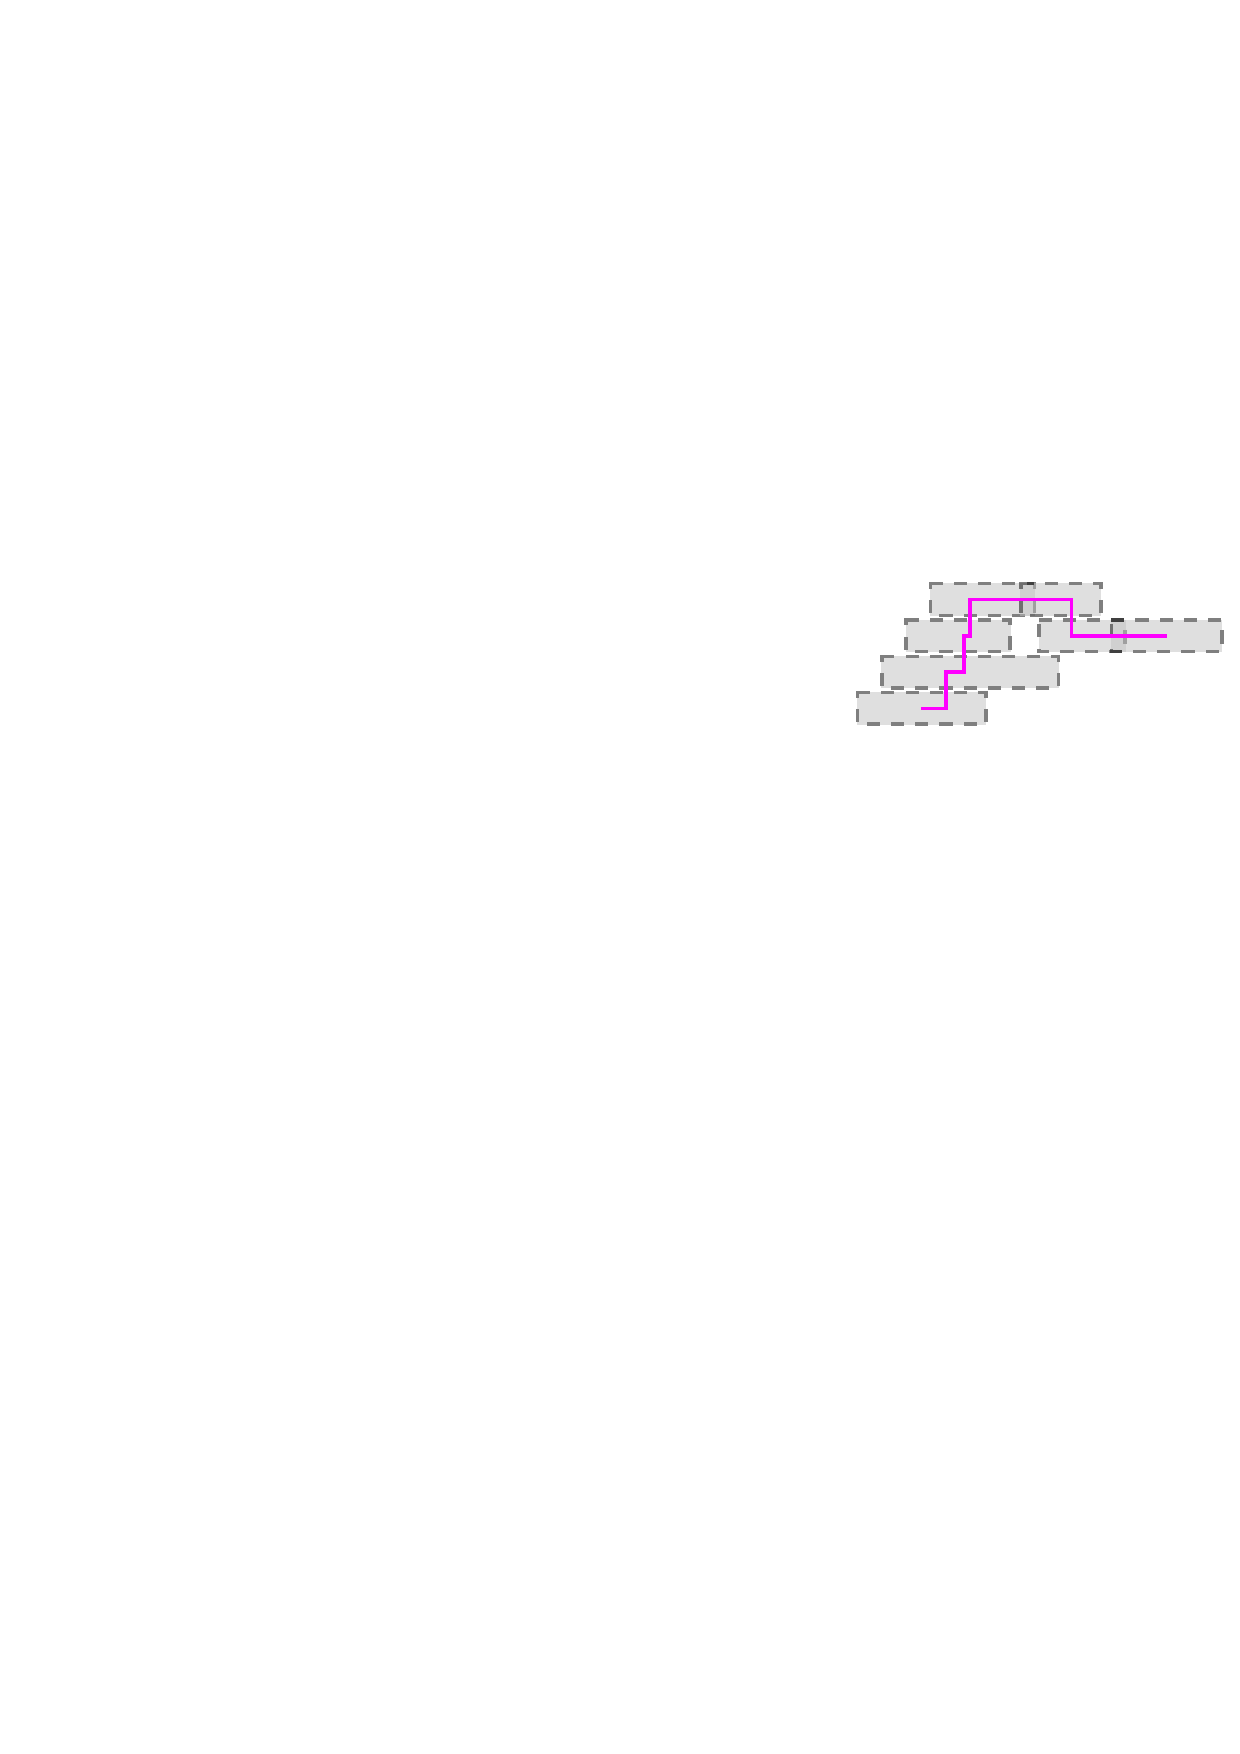
\includegraphics[width=.47\linewidth]{figure9b}}
\caption{Layer layout algorithms. Each rectangle represents an event. The line connecting centers of rectangles illustrates the  traceability.}
\label{fig:traceability}
\end{figure}

\subsection{Layers Compacting}
\label{sub:compact}
The aforementioned layer layout needs a maximum number of rows it can use as an input. Initially, it is assigned proportionally to the number of events within each layer. After the layout of each layer is independently computed, some sets may need to move to fill the new space that appears between layers. This includes moving two layers closer if there is a gap in between, or moving a layer into a newly created space if its set does not share events with any other sets. The freed space is assigned to the layer with the lowest completeness ratio $\theta$. Then, layouts of all layers are recomputed and compacted again. The process repeats until no more space can be saved. Figure~\ref{fig:compacting} shows an example of compacting. 

\begin{figure}[!htb]
	\centering
	\subcaptionbox{Before compacting.}{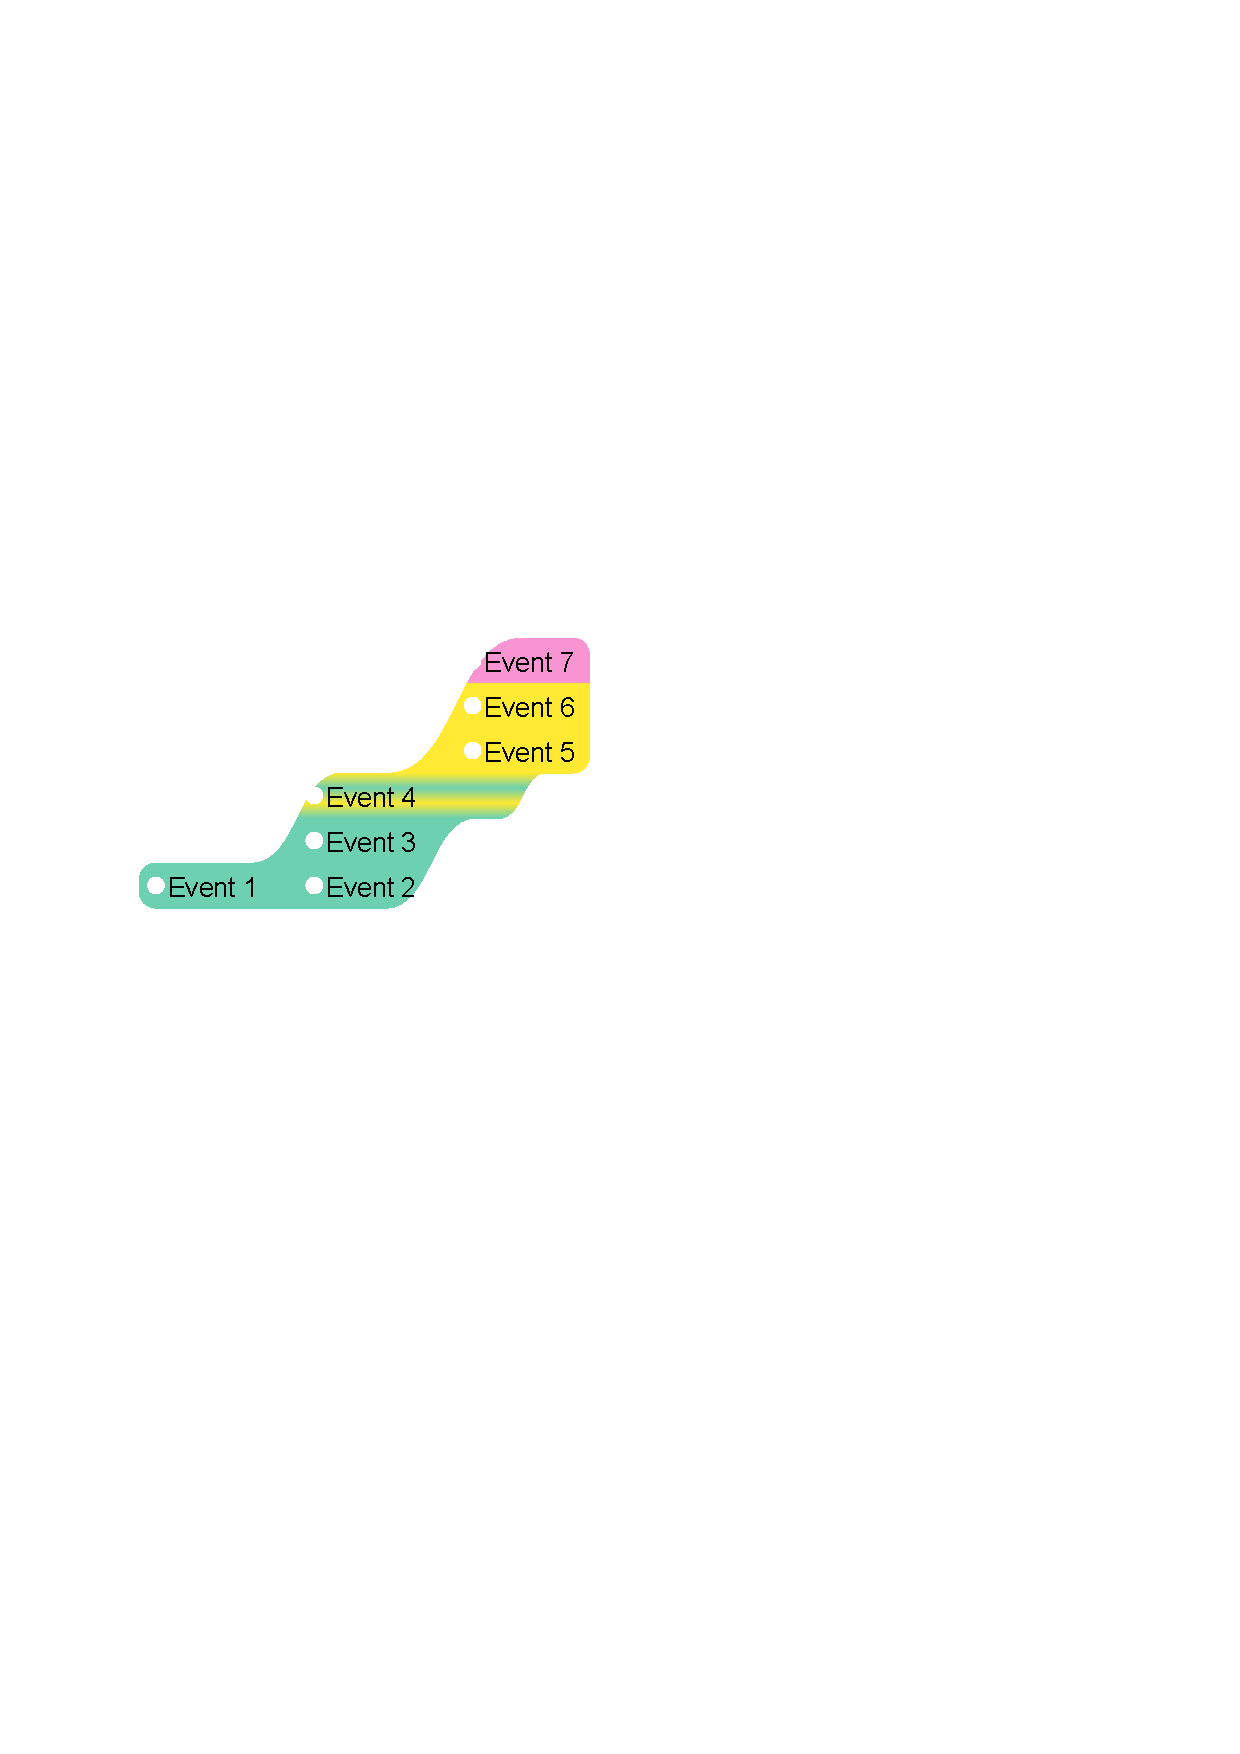
\includegraphics[width=.47\columnwidth]{figure10a}}
	\hfill
	\subcaptionbox{After compacting.}{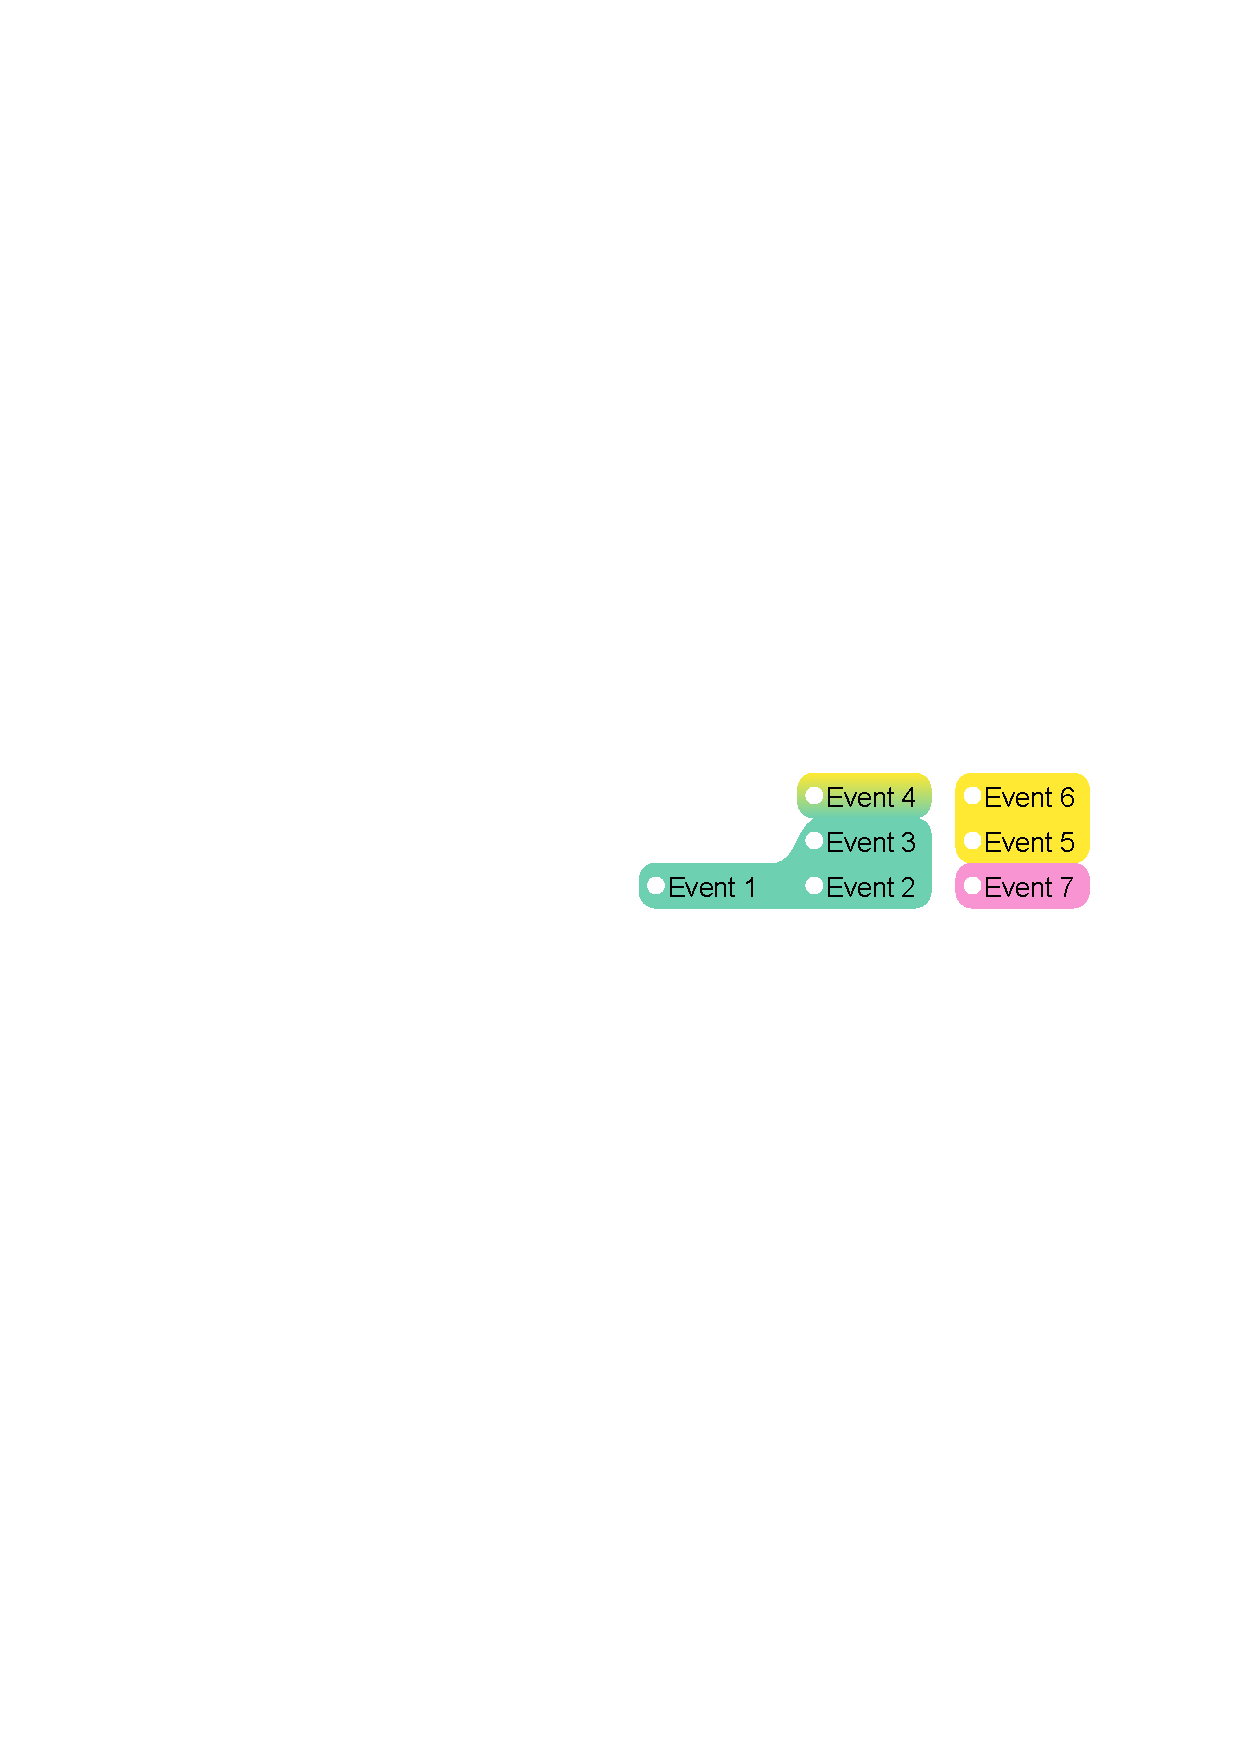
\includegraphics[width=.47\columnwidth]{figure10b}}
	\caption{Layers compacting.}
	\label{fig:compacting}
\end{figure}

\subsection{Layers Balancing}
This last step ensures that all layers have similar levels of detail; i.e., avoiding layers with many complete events and other layers with many aggregated events. This is achieved by minimizing the variance of completeness ratios of all layers, 
$\frac{\sum\limits_{i=1}^{n}(\theta_i - \bar{\theta})^2} {n}$, where $n$ is the number of layers and $\bar{\theta}$ is the mean of all completeness ratios. A brute force approach tests all possible combinations of layer height $h_i$ such that $\sum\limits_{i=1}^{n}h_i=H$ for a minimum variance, where $H$ is the height of the display area. However, the number of combinations is an exponential of $n$. Instead, we apply a heuristic algorithm that relies on a simple observation that the completeness ratio increases with layer height. Therefore, the algorithm reduces the completeness ratio variance by iteratively transferring a row from the layer with the largest ratio to the layer with the smallest one, until the variance no longer decreases. Figure~\ref{fig:balancing} shows an example of balancing.

\begin{figure}[!htb]
	\centering
	\subcaptionbox{Before balancing: $\theta_{green}=0.25$, $\theta_{yellow}=1$.}{\label{fig:balancing1}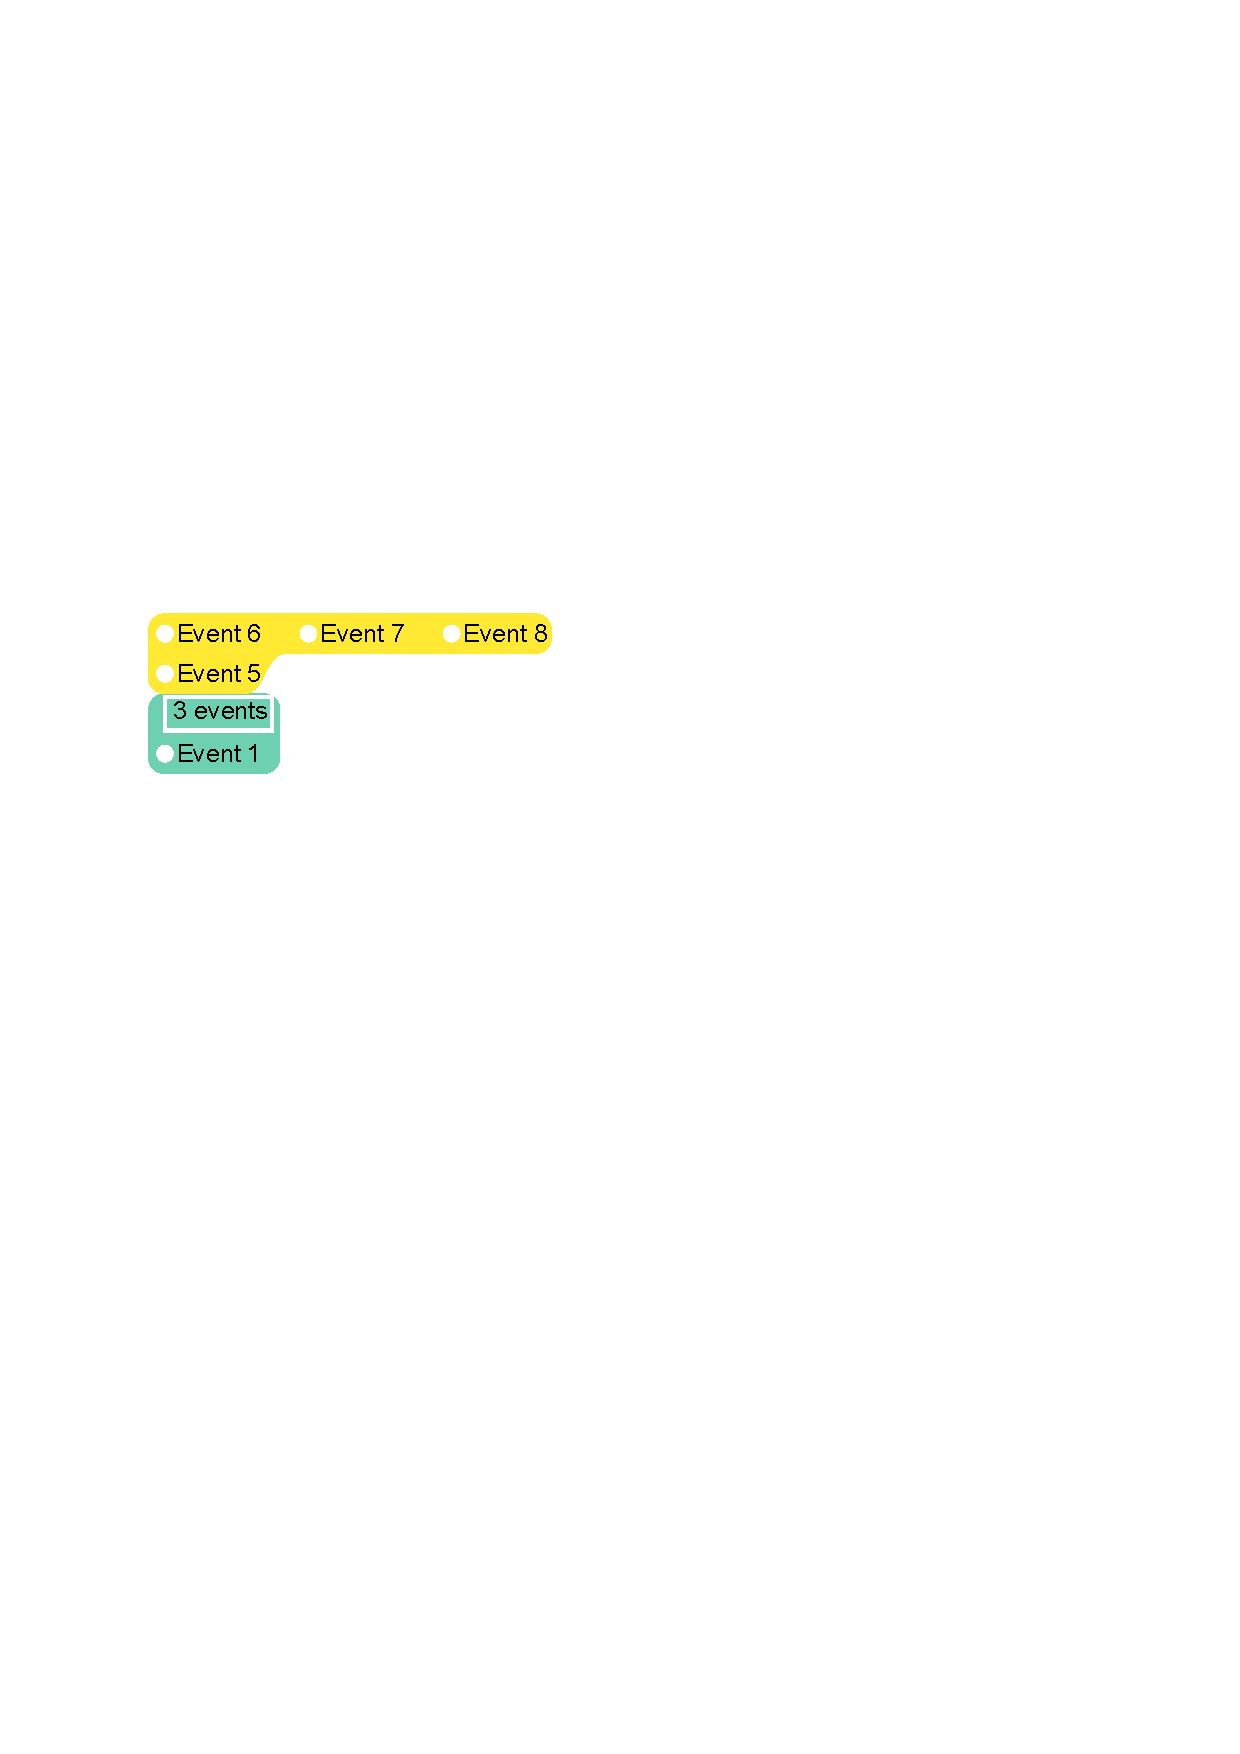
\includegraphics[width=.48\columnwidth]{figure11a}}
	\hfill
	\subcaptionbox{After balancing: $\theta_{green}=\theta_{yellow}=0.5$.}{\label{fig:balancing2}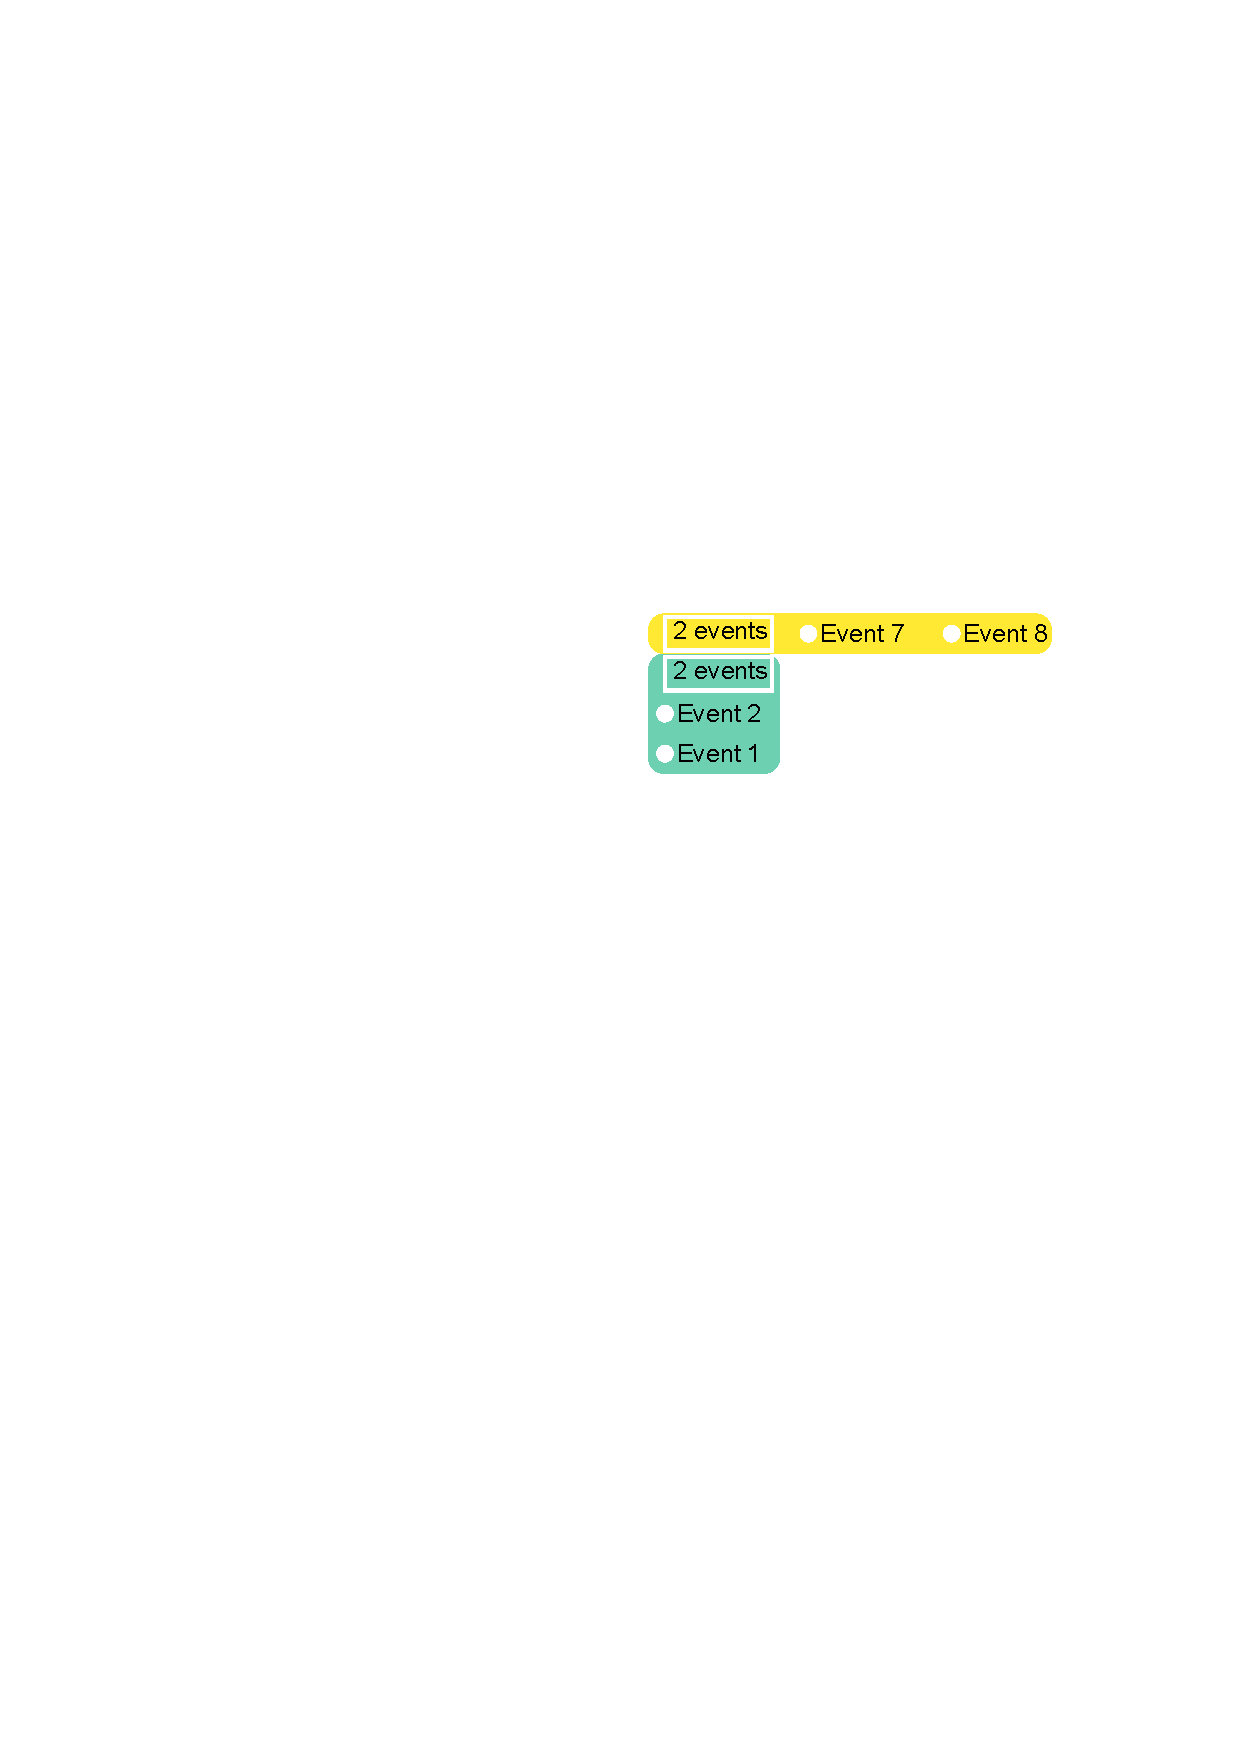
\includegraphics[width=.48\columnwidth]{figure11b}}
	\caption{Layers balancing.}
	\label{fig:balancing}
\end{figure}

\subsection{Scalability}
Aggregation enables TimeSets to visualize a large number of events. However, the visual representation of aggregated events is imperfect. For instance, two aggregates ``2 events'' and ``100 events'' are displayed exactly the same, except for the total number, whereas their sizes are largely different. We consider four options to address this issue as shown in Figure~\ref{fig:aggreate}. 

The first option is to plot each individual event as a dot at when it happens (Figure~\ref{fig:aggregate-1}). This also provides a temporal distribution of events rather than just the total count. When events happen closely, dots are overlapped, which makes it more difficult to see the pattern. Second, the width of the rectangular border can be scaled to indicate the number of events (Figure~\ref{fig:aggregate-1}). The full width of an aggregate border is typically small as the length of text ``$N$ events''. Therefore, the difference among aggregate border widths could be subtle and difficult to observe from an overview. Another option is to color code the background of the bounding rectangle using luminance or intensity (Figure~\ref{fig:aggregate-3}) according to the number of events. However, when many aggregated events are displayed, their backgrounds could interfere with the set colors and distract users. The last option we propose is to scale the font size of the label based on the number of events (Figure~\ref{fig:aggregate-4}). Currently, each event is completely located in one single row with uniform height. Scaling the heights of aggregated events will affect the layout algorithm. 

\note{move this section to Discussion of the chapter?}
All these methods have their strengths and limitations, thus deciding the best one is challenging and out of scope for this paper. We leave the implementation and evaluation of these methods as future work.

\begin{figure}[!htb]
	\centering
	\subcaptionbox{No encoding.\label{fig:aggregate-0}}{
		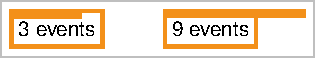
\includegraphics[width=.47\columnwidth]{figure12a}}
	\\
	\subcaptionbox{Scale with the width of the bounding rectangle.\label{fig:aggregate-1}}{
		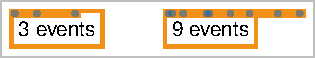
\includegraphics[width=.47\columnwidth]{figure12b}}
	\hfill
	\subcaptionbox{Each dot is an event at when it happens.\label{fig:aggregate-2}}{
		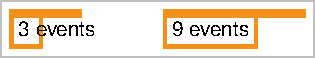
\includegraphics[width=.47\columnwidth]{figure12c}}
	\\
	\subcaptionbox{Color code the background of the bounding rectangle.\label{fig:aggregate-3}}{
		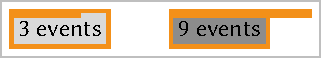
\includegraphics[width=.47\columnwidth]{figure12d}}
	\hfill
	\subcaptionbox{Scale with the font size of the label.\label{fig:aggregate-4}}{
		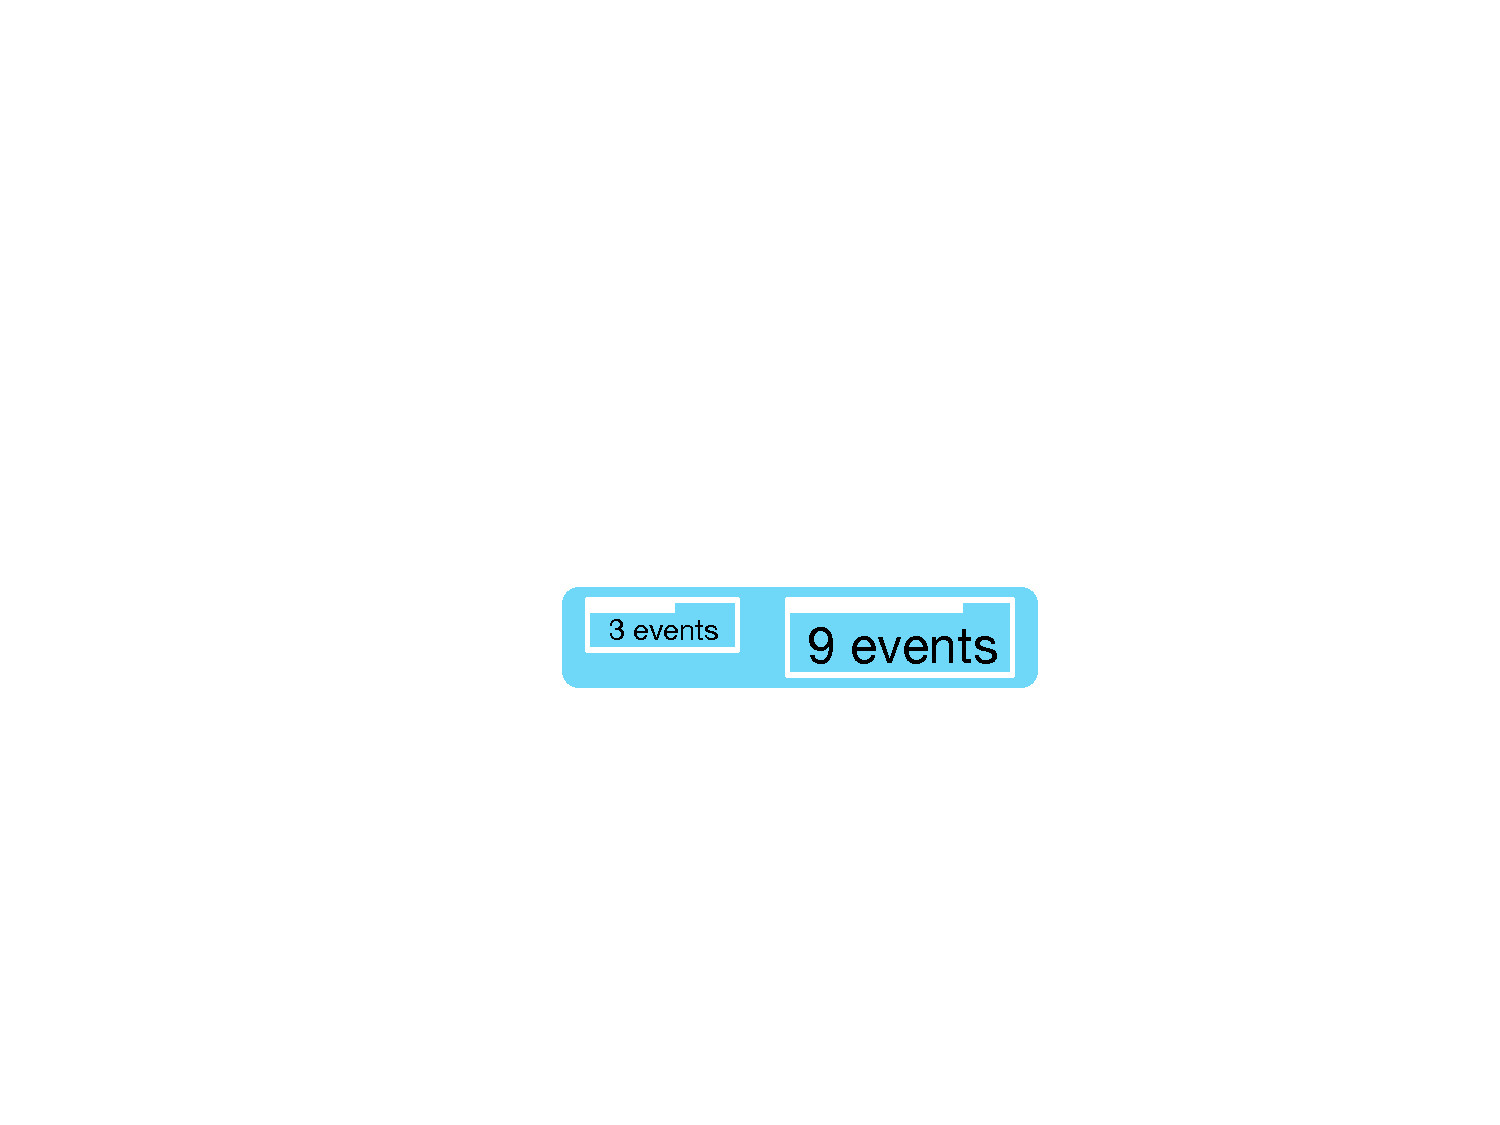
\includegraphics[width=.47\columnwidth]{figure12e}}
	\caption{Proposed visual representations of aggregates emphasizing the number of its events.}
	\label{fig:aggreate}
\end{figure}

The existing layout is suitable for a small timeline with a few hundreds of events or a detailed view where individual events are of high importance. Figure~\ref{fig:citations} shows 225 publications within 15 years. TimeSets relies on color to distinguish sets, therefore it is constrained by the number of colors that human can differentiate at the same time, which is about 12, according to Munzner's book~\cite{Munzner2014}.